%% Phase 2 report -- CSCE 3602 / DSCI 3415 Fundamentals of Machine Learning
%% AI was used to help format this report, but the text was written and reviewed by the authors.
\documentclass[sigconf,nonacm,10pt]{acmart}
\usepackage{tabularx}
\usepackage{booktabs}
\sloppy
\settopmatter{printacmref=false}
\setcopyright{none}
\renewcommand\footnotetextcopyrightpermission[1]{}
\pagestyle{plain}

\begin{document}

\title{Fair Price in a Moving Market: Predicting Residential Prices}
\subtitle{Phase 2: Data Preparation, Cleaning and Feature Generation}

\author{Zeyad Khaled}
\affiliation{%
  \institution{The American University in Cairo}
  \city{Cairo}
  \country{Egypt}}

\author{Mohamed Akram}
\affiliation{%
  \institution{The American University in Cairo}
  \city{Cairo}
  \country{Egypt}}

\begin{abstract}
This report aims to explore data set preparation for our machine learning project. The initial data set chosen was in the context of Egyptian real estate prices, but after instructor feedback we replaced it with the Zillow Prize (Zestimate) property dataset from Kaggle, which fit the required parameters. After pre-processing and cleaning we obtained 12 features. We used statistical inference to clean data, replace missing values and scale features in order to obtain a clean dataset of 2,950,951 records with no missing values to use for a linear regression model. The label being predicted is \texttt{taxvaluedollarcnt}.
\end{abstract}

\keywords{data cleaning, feature generation, encoding, missing values, scaling}

\maketitle

\section{Dataset Size}

The original size was 2,985,217 rows and 58 columns. After removing the 34,266 rows with a missing label, we have 2,950,951 rows and 48 columns. These columns include 7 numeric and 5 categorical feature columns, in addition to all the one-hot encoding and frequency encoding columns.

\section{Dropped Columns}

\subsection{Leakage}

\begin{table}[h]
\caption{Columns dropped because they leak the label.}
\small
\begin{tabularx}{\columnwidth}{@{}lX@{}}
\toprule
Column & Why \\
\midrule
\texttt{structuretaxvaluedollarcnt} & Addition with another column gives the label, so leaking occurs \\
\texttt{landtaxvaluedollarcnt} & Addition with another column gives the label, so leaking occurs \\
\texttt{taxamount} & Addition with another column gives the label, so leaking occurs \\
\bottomrule
\end{tabularx}
\end{table}

\subsection{High missingness, and no way to find what the missing values represent}

\begin{table*}[t]
\caption{Columns dropped for high missingness.}
\footnotesize
\begin{tabularx}{\textwidth}{@{}p{2.9cm}>{\raggedright\arraybackslash}p{6.0cm}>{\raggedright\arraybackslash}X@{}}
\toprule
Subgroup & Columns & Why \\
\midrule
Pool and spa (6) & \texttt{poolcnt}, \texttt{poolsizesum}, \texttt{pooltypeid2}, \texttt{pooltypeid7}, \texttt{pooltypeid10}, \texttt{hashottuborspa} & Close to 99\% missing rows; inadequate pool information of any kind to build a feature \\
\addlinespace
Fireplace, garage, deck (5) & \texttt{fireplacecnt}, \texttt{fireplaceflag}, \texttt{garagecarcnt}, \texttt{garagetotalsqft}, \texttt{decktypeid} & \texttt{fireplacecnt} 89.51\% missing, garage columns above 70\%; \texttt{decktypeid} 99.42\% missing with a single observed category (66), so no variation \\
\addlinespace
Building structure (11) & \texttt{airconditioningtypeid}, \texttt{architecturalstyletypeid}, \texttt{buildingclasstypeid}, \texttt{basementsqft}, \texttt{storytypeid}, \texttt{typeconstructiontypeid}, \texttt{threequarterbathnbr}, \texttt{numberofstories}, \texttt{yardbuildingsqft17}, \texttt{yardbuildingsqft26}, \texttt{unitcnt} & \texttt{basementsqft} is 99.95\% missing; \texttt{threequarterbathnbr} is also just one component of the bathroom total; \texttt{unitcnt} is not over the missingness threshold, but \texttt{propertylandusetypeid} already gives us the information needed and it has fewer missing rows. The other columns are over the threshold \\
\addlinespace
Tax delinquency (2) & \texttt{taxdelinquencyflag}, \texttt{taxdelinquencyyear} & 98.1\% missing, and also removed for semantic reasons, as these columns have to do with the owner's behaviour \\
\addlinespace
Zoning and census identifiers (2) & \texttt{propertyzoningdesc}, \texttt{censustractandblock} & \texttt{propertyzoningdesc} has thousands of codes, so encoding is difficult, and \texttt{propertylandusetypeid} and \texttt{propertycountylandusecode} are already sufficient; \texttt{censustractandblock} is a long geographic identifier, not a quantity, and location is covered by \texttt{fips}, latitude and longitude \\
\bottomrule
\end{tabularx}
\end{table*}

\subsection{Redundant with a kept feature (13)}

\begin{table*}[t]
\caption{Columns dropped as redundant.}
\footnotesize
\begin{tabularx}{\textwidth}{@{}>{\raggedright\arraybackslash}p{7.5cm}>{\raggedright\arraybackslash}X@{}}
\toprule
Column & Why \\
\midrule
\texttt{calculatedbathnbr} & Follows \texttt{bathroomcnt} in 100\% of cases, but it has more missing values \\
\texttt{fullbathcnt} & Follows \texttt{bathroomcnt} \\
\texttt{finishedfloor1squarefeet}, \texttt{finishedsquarefeet12}, \texttt{13}, \texttt{15}, \texttt{50}, \texttt{6} & Redundant with the feature \texttt{calculatedfinishedsquarefeet}, which is kept \\
\texttt{rawcensustractandblock}, \texttt{regionidcity}, \texttt{regionidcounty}, \texttt{regionidneighborhood}, \texttt{regionidzip} & Location is already represented by \texttt{fips}, latitude and longitude; the encodings would be large and would just show the same data \\
\bottomrule
\end{tabularx}
\end{table*}

\subsection{Not useful}

\begin{table}[h]
\caption{Columns dropped for carrying no usable signal.}
\small
\begin{tabularx}{\columnwidth}{@{}lX@{}}
\toprule
Column & Why \\
\midrule
\texttt{parcelid} & A unique identifier does not contribute \\
\texttt{assessmentyear} & Most values are the same \\
\texttt{roomcnt} & 77.6\% recorded as zero rooms, so we use bathroom count and bedroom count as better indicators \\
\bottomrule
\end{tabularx}
\end{table}

\section{Kept Features}

\subsection{Numeric}

\begin{table*}[t]
\caption{The seven numeric features that were kept.}
\footnotesize
\setlength{\tabcolsep}{4pt}
\begin{tabular}{@{}lrrrrrrrrr@{}}
\toprule
Feature & Missing & Unique & Min & Median & Mean & Max & Std & Skew & Correlation \\
\midrule
\texttt{bathroomcnt} & 0.099\% (2,957) & 39 & 0 & 2 & 2.22 & 32 & 1.08 & 1.18 & 0.308 \\
\texttt{bedroomcnt} & 0.099\% (2,945) & 25 & 0 & 3 & 3.09 & 25 & 1.27 & 0.50 & 0.138 \\
\texttt{yearbuilt} & 1.60\% (47,833) & 183 & 1801 & 1963 & 1964.4 & 2016 & 23.6 & $-0.15$ & 0.130 \\
\texttt{calculatedfinishedsquarefeet} & 1.51\% & 12,631 & 1 & 1,574 & 1,831 & 952,576 & 1,954 & 156.4 & 0.560 \\
\texttt{lotsizesquarefeet} & 9.14\% (272,706) & 70,214 & 100 & 7,000 & 22,604 & 371,000,500 & 249,984 & 1,208.5 & 0.005 \\
\texttt{latitude} (degrees) & 0.098\% (2,932) & 852,718 & 33.324 & 34.008 & 34.001 & 34.820 & 0.244 & 0.28 & $-0.057$ \\
\texttt{longitude} (degrees) & 0.098\% (2,932) & 1,043,238 & $-119.476$ & $-118.172$ & $-118.202$ & $-117.554$ & 0.346 & $-0.78$ & $-0.020$ \\
\bottomrule
\end{tabular}
\end{table*}

\begin{itemize}
\item \texttt{bathroomcnt}: low number of missing values, and the median rises with the number of bathrooms.
\item \texttt{bedroomcnt}: a steady increase in value with increasing rooms is observed.
\item \texttt{yearbuilt}: gives property age, so it has semantic importance.
\item \texttt{calculatedfinishedsquarefeet}: a strong correlation is observed.
\item \texttt{lotsizesquarefeet}: adds land-related semantic information.
\item \texttt{latitude} and \texttt{longitude}: finer location parameters that work with \texttt{fips}.
\end{itemize}

\subsection{Categorical}

\begin{table*}[t]
\caption{The five categorical features that were kept.}
\footnotesize
\begin{tabularx}{\textwidth}{@{}p{3.4cm}p{2.4cm}p{2.3cm}p{4.2cm}X@{}}
\toprule
Feature & Missing & Unique & Largest categories & Encoding \\
\midrule
\texttt{buildingqualitytypeid} & 34.97\% (1,043,822) & 12 & 6 (561,502), 8 (501,925), 4 (448,049) & One-hot, missing as ``Unknown'' \\
\texttt{fips} & 0.098\% (2,932) & 3 & 6037 (67.4\%), 6059 (25.0\%), 6111 (7.5\%) & One-hot, missing as ``Unknown'' \\
\texttt{heatingorsystemtypeid} & 37.39\% (1,116,053) & 14 & 2 (1,168,610), 7 (646,021) & Identifiers mapped to heating-system names, then one-hot, missing as ``Unknown'' \\
\texttt{propertylandusetypeid} & 0.098\% (2,932) & 16 (15 after label removal) & 261 (72.1\%), 266 (16.2\%) & One-hot, missing as ``Unknown'' \\
\texttt{propertycountylandusecode} & 0.10\% (2,999) & 234 & 0100 (1,153,332), 122 (522,127), 0101 (248,386) & Frequency encoding, missing as ``Unknown'' \\
\bottomrule
\end{tabularx}
\end{table*}

\begin{itemize}
\item \texttt{buildingqualitytypeid}: each quality shows up with a different value, so it does contribute.
\item \texttt{fips}: geographical information is a big factor in real estate pricing.
\item \texttt{heatingorsystemtypeid}: different values for different identifiers, so it does contribute.
\item \texttt{propertylandusetypeid}: value differences are observed.
\item \texttt{propertycountylandusecode}: a low number of missing values, and more detailed than \texttt{propertylandusetypeid}.
\end{itemize}

\section{Transformations}

\subsection{Categorical encodings}

\textbf{One-hot (4 features):} \texttt{buildingqualitytypeid}, \texttt{fips},
\texttt{heatingorsystemtypeid} and \texttt{propertylandusetypeid}. The identifiers are just
identifiers and the numbers themselves do not hold any actual weight, so one-hot encoding is used.

\textbf{Frequency encoding (1 feature):} the column
\texttt{propertycountylandusecode}. With 234 categories, one-hot would add too many columns, so we use frequency encoding instead. The limitation with regard to collisions is noted.

\subsection{Numeric transformations}

\begin{itemize}
\item \textbf{Median imputation:} for \texttt{bathroomcnt}, \texttt{bedroomcnt} and \texttt{yearbuilt}.
\item \textbf{Divide by 1,000,000, then median imputation:} \texttt{latitude} and \texttt{longitude}, because Zillow stores coordinates scaled by $10^6$.
\item \textbf{Log, then median imputation:} \texttt{calculatedfinishedsquarefeet} and \texttt{lotsizesquarefeet}, because of large skewness.
\item \textbf{Z-score on 8 numeric columns:} bathrooms, bedrooms, year built, log finished area, log lot size, latitude, longitude, and the frequency-encoded county code.
\end{itemize}

\section{Figures}

\begin{figure}[h]
\centering
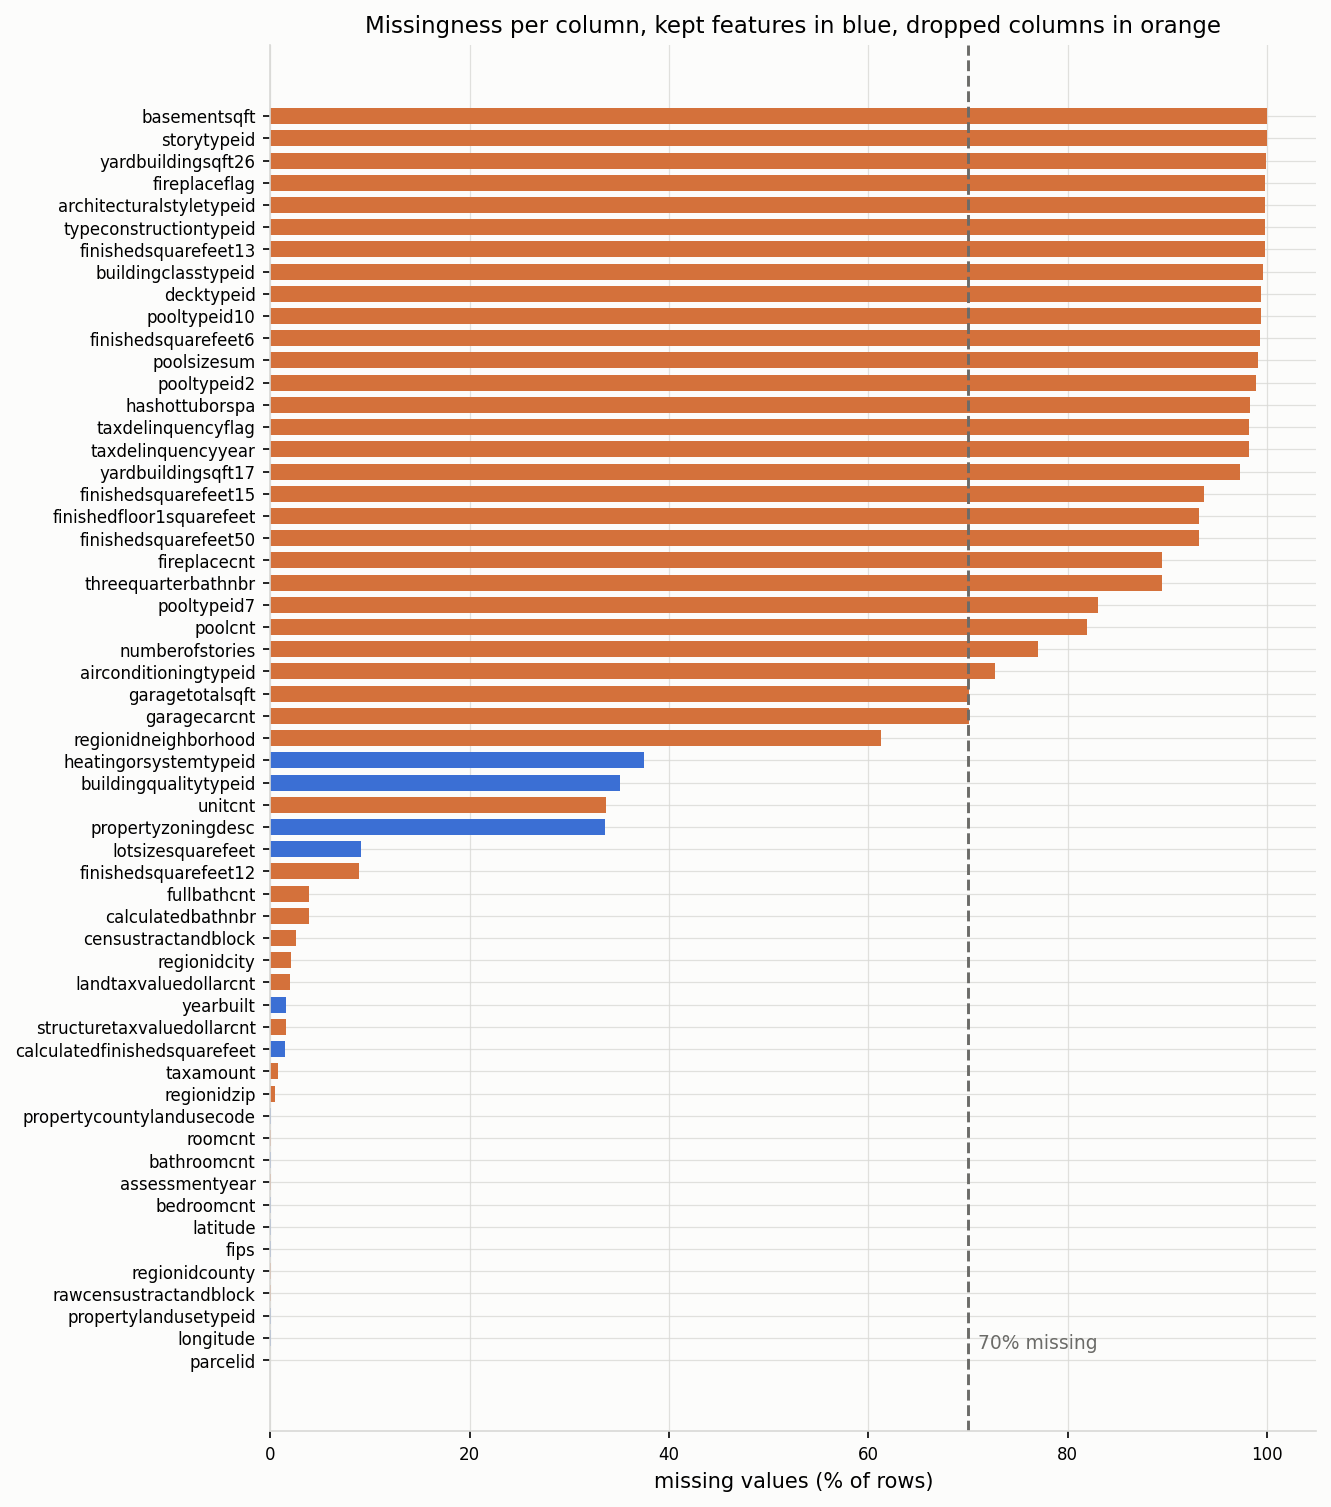
\includegraphics[width=\columnwidth]{../figures/fig1_missingness.png}
\caption{Missingness per column. Kept features are in blue and dropped columns in orange.}
\end{figure}

\begin{figure}[h]
\centering
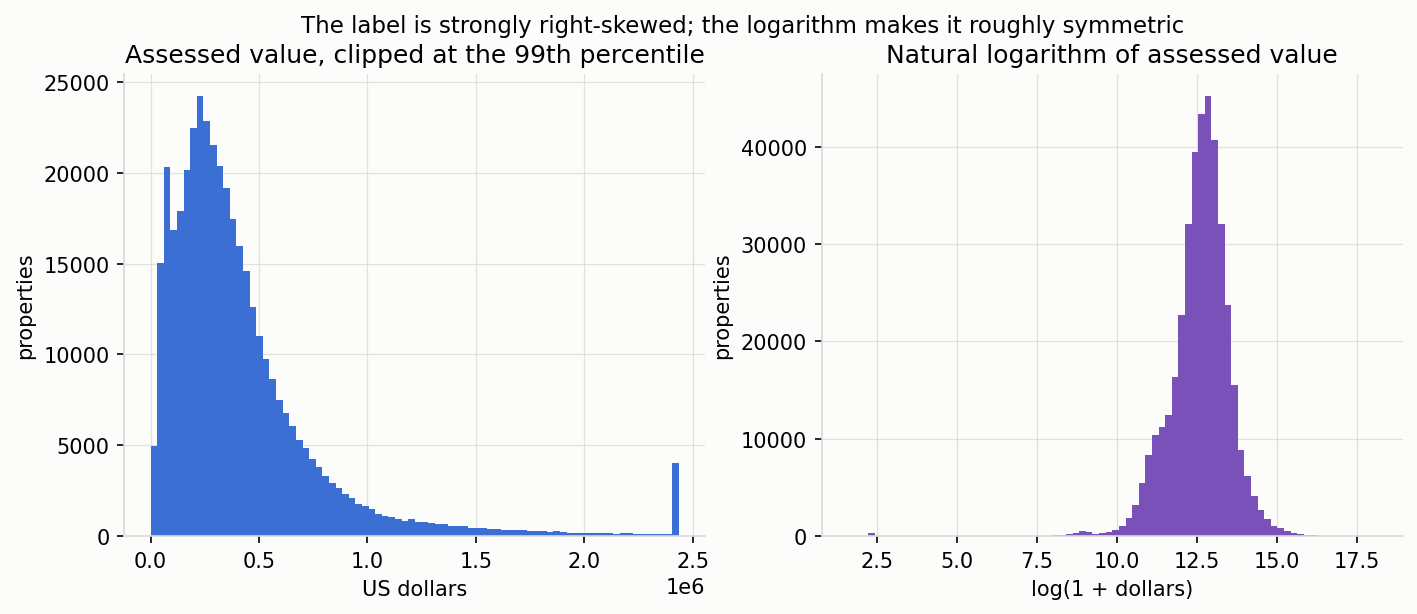
\includegraphics[width=\columnwidth]{../figures/fig2_label_distribution.png}
\caption{The label before and after a logarithm.}
\end{figure}

\begin{figure}[h]
\centering
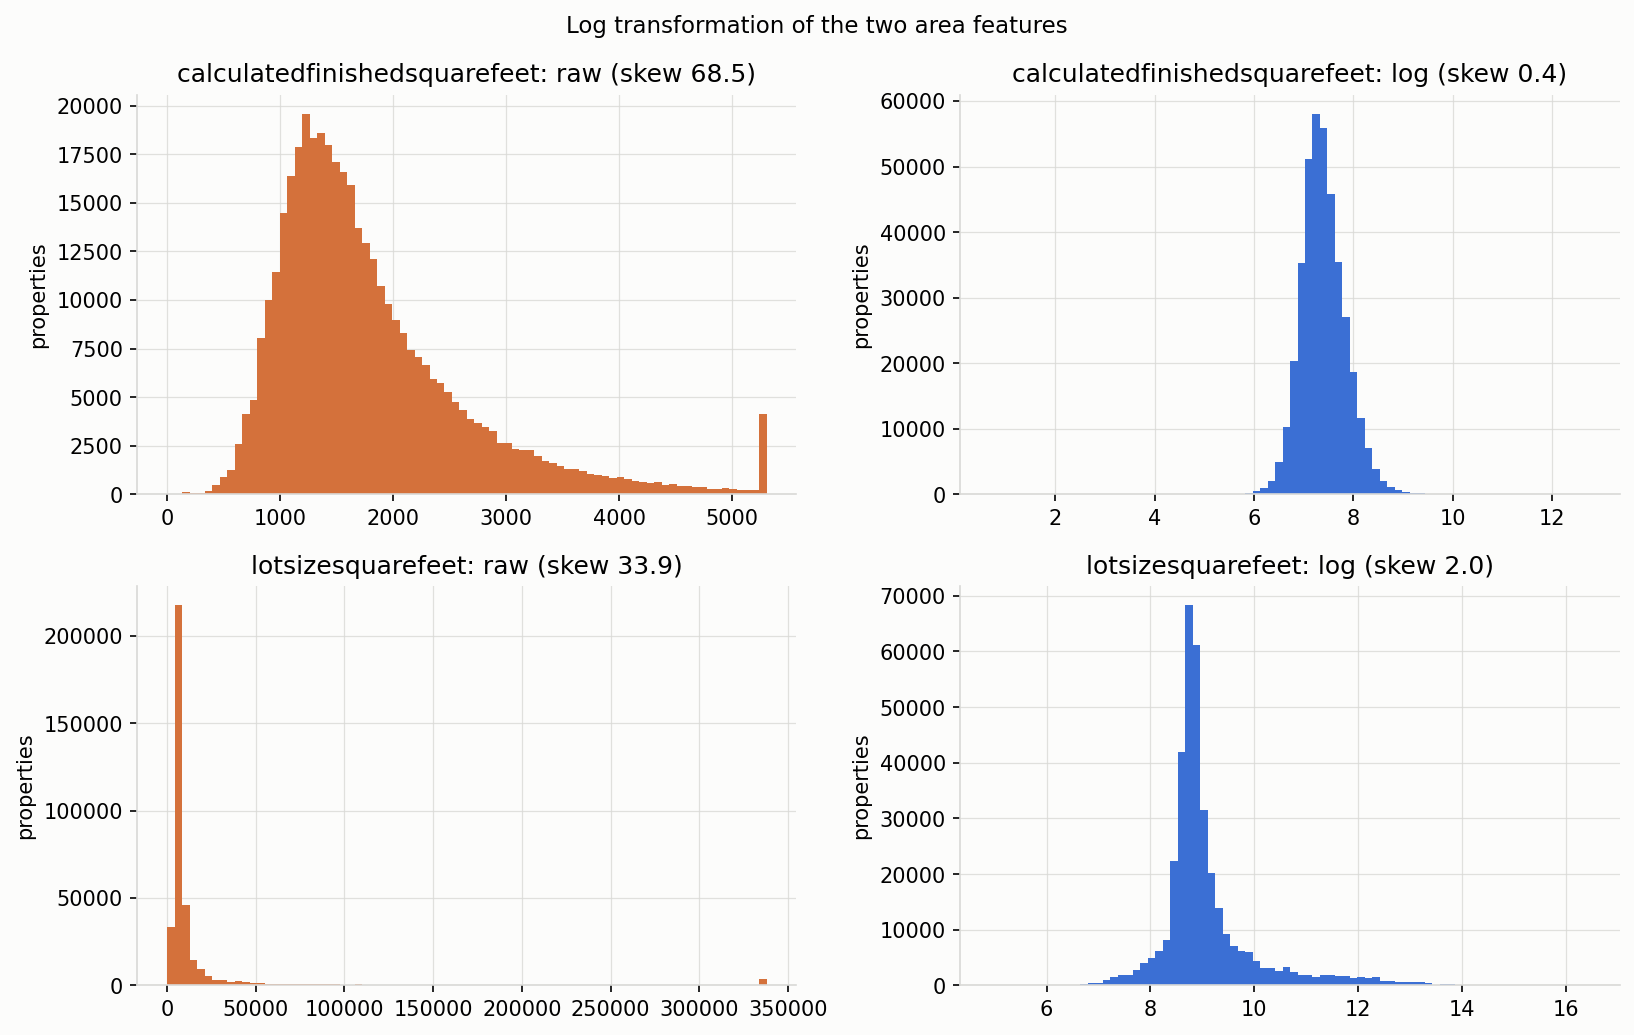
\includegraphics[width=\columnwidth]{../figures/fig3_area_transformations.png}
\caption{The two area features before and after the logarithm, with the skew of each.}
\end{figure}

\begin{figure}[h]
\centering
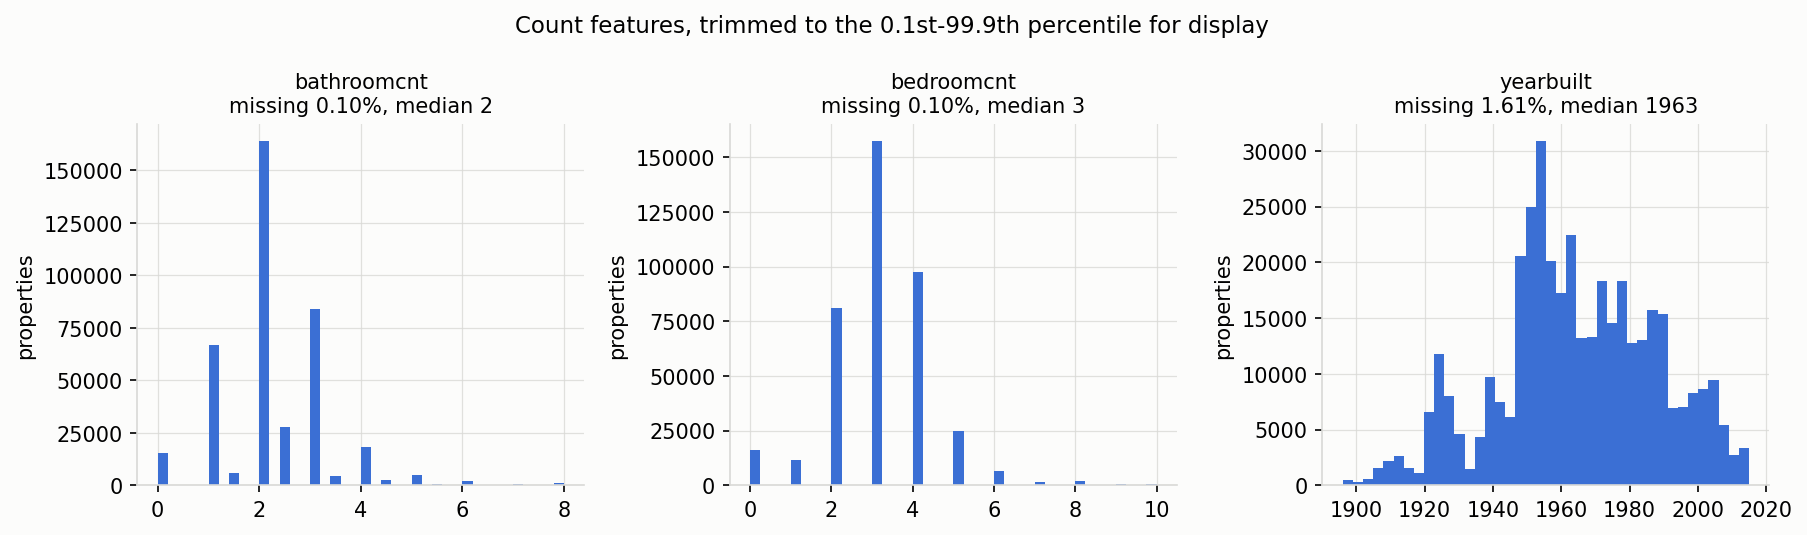
\includegraphics[width=\columnwidth]{../figures/fig4_count_distributions.png}
\caption{The three count features, with their missingness and median.}
\end{figure}

\begin{figure}[h]
\centering
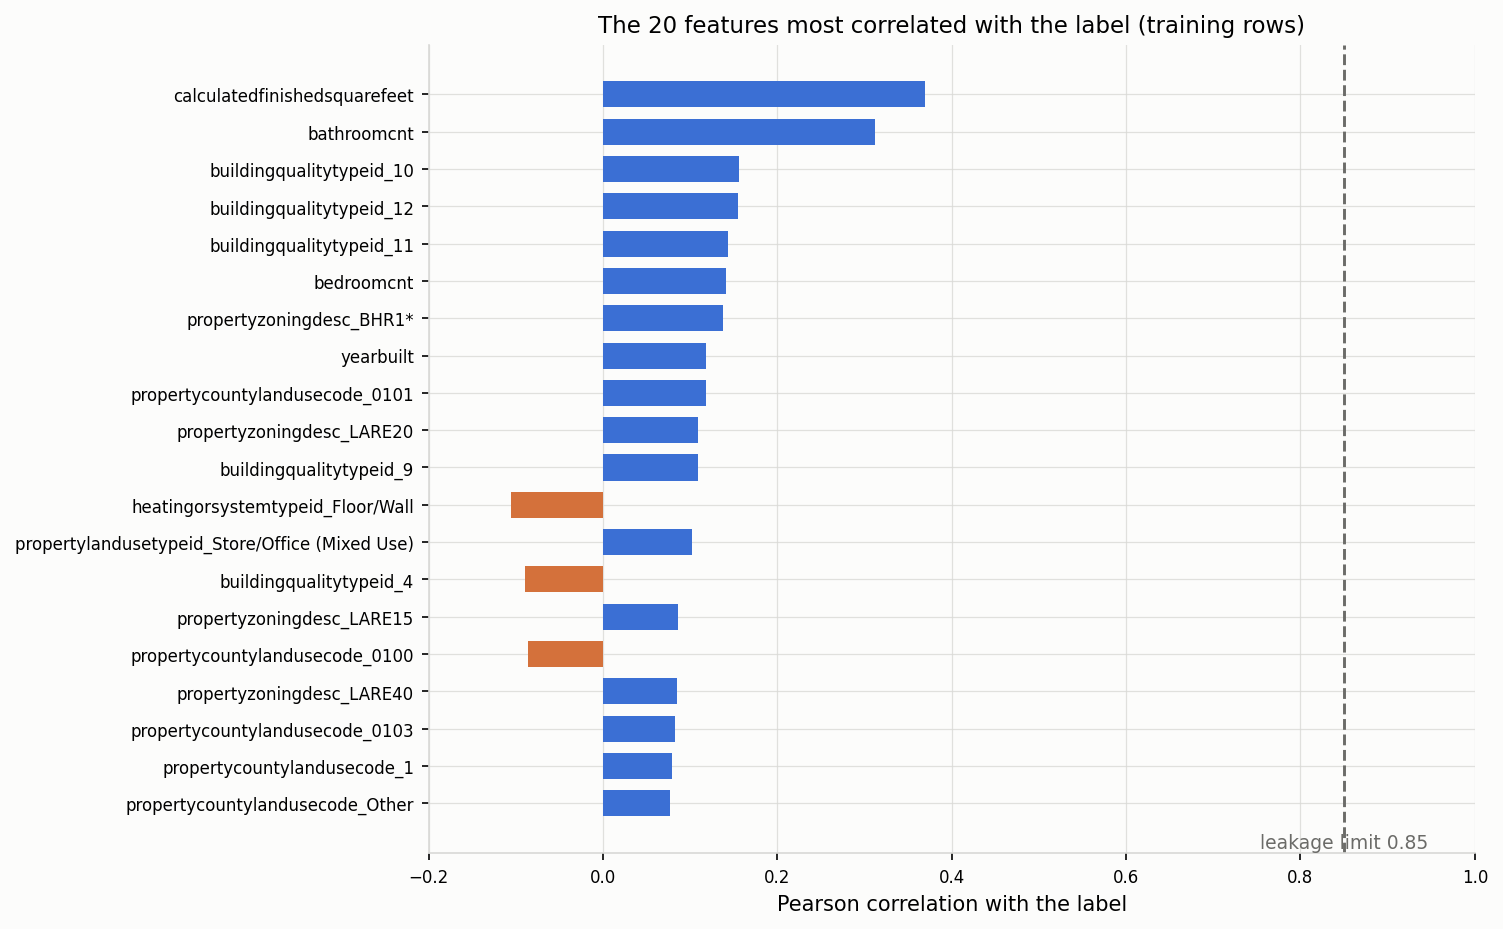
\includegraphics[width=\columnwidth]{../figures/fig5_label_correlation.png}
\caption{The strongest correlations with the label, against the 0.85 limit.}
\end{figure}

\begin{figure}[h]
\centering
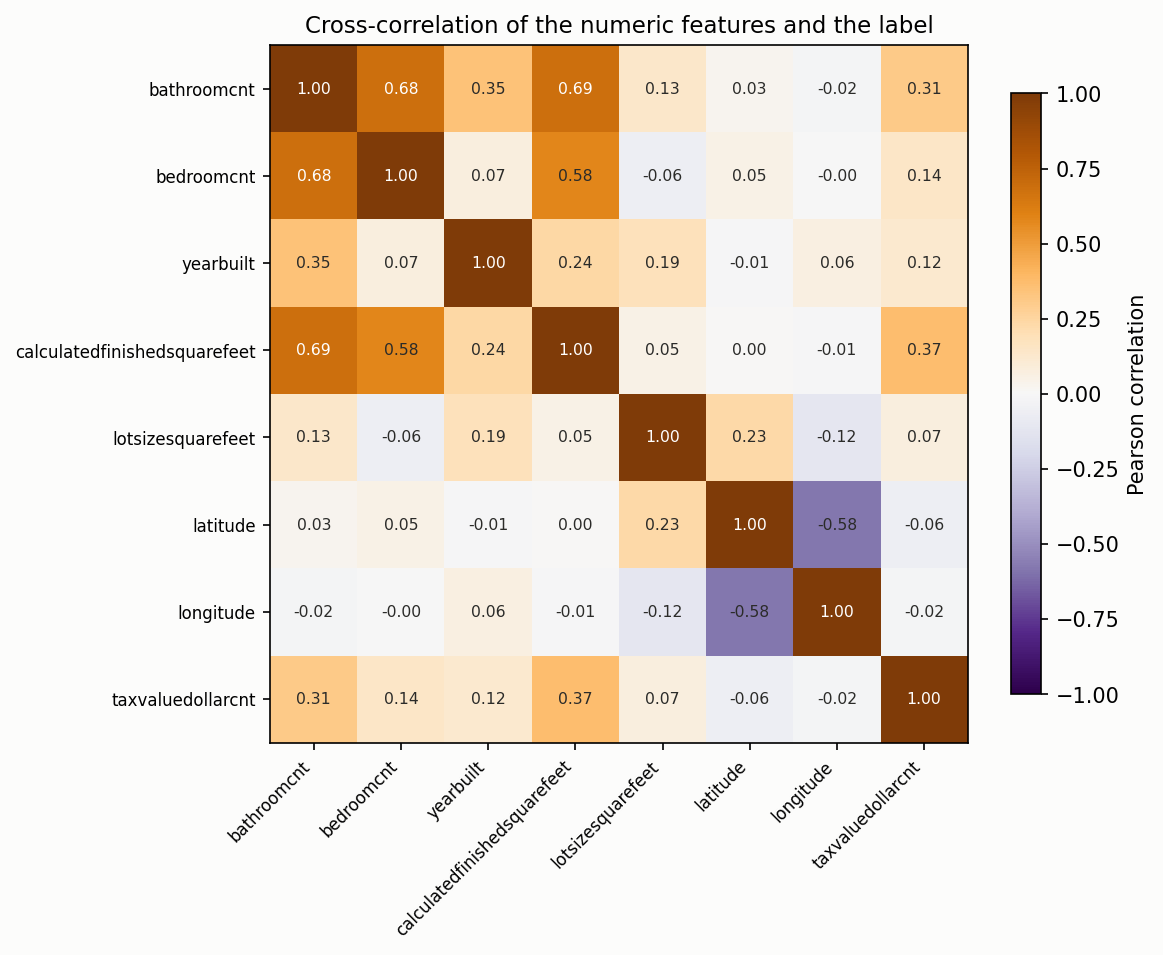
\includegraphics[width=\columnwidth]{../figures/fig6_cross_correlation.png}
\caption{Cross-correlation of the numeric features and the label.}
\end{figure}

\begin{figure}[h]
\centering
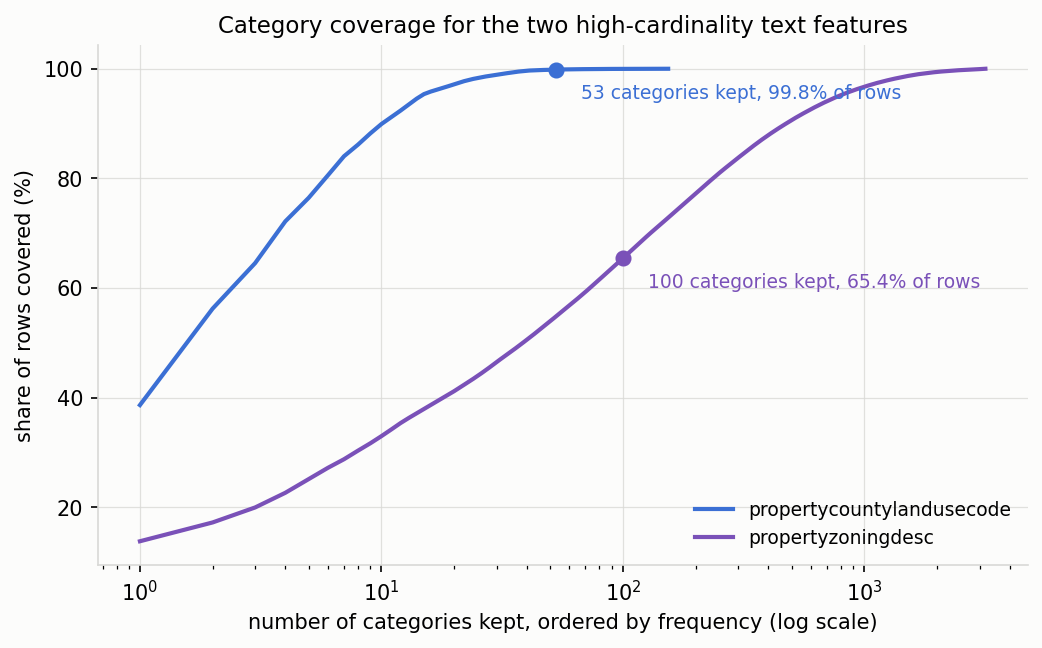
\includegraphics[width=\columnwidth]{../figures/fig7_category_coverage.png}
\caption{How many categories are needed to cover most of the rows.}
\end{figure}

\end{document}
